\chapter{Task 1}
% TODO How is the element notated graphically or textually
\section{UML Model elements}
All the visual notation for the elements listed below are present in this picture:
\begin{figure}[hbt]
\label{Class}
  \centering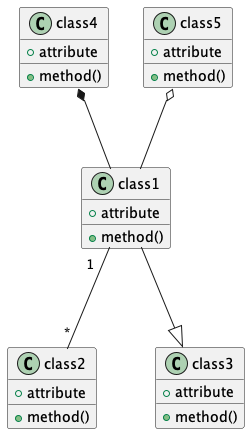
\includegraphics[width=0.4\textwidth]{Immagini/test-3.png}
  \caption{Class}
\end{figure}


\subsection{Class}
A class represents an abstraction of a collection of objects (equally treated as the type of the same collection of objects). Class is the modeling and programming entity, that is instantiated later into a set of objects at run-time. The objects instantiated from a particular class will all behave identically; these behaviours are defined by the methods (or operations) of the class. The structure of a class is defined by a set of attributes which also characterizes the state of an object instantiated from the class.\\

A class may have an optional qualifier. If specified, the qualifier is generally one of the attributes of the class. The qualifier is used to identify a unique object/instance of the class when multiple objects/instances are used in a relationship with another class.\\

The name of the class must be present. The attributes and methods of the class need not be shown in the diagram. Even if they are specified, they do not need to be fully specified in the diagram. However, for verification with respect to the application domain, complete details of all attributes and methods are needed. These can be specified in a separate document outside the class diagram.\\
Each class has a unique name within the diagram.  If a class name appears more than once in the same diagram, then logically these icons are combined into one.\\
The class name compartment may also include additional information such as whether or not the class is abstract, persistent, author information etc. \\
 A class icon may or may not have attributes or operations.
 The name of an attribute is unique within the class.\\
 A method is uniquely identified by its signature. Thus, overloaded methods may have the same names but different signatures.\\
 The set of names of attributes and the set of names of methods are mutually exclusive.\\
 No attribute can have the same name as that of the class. However, constructor methods may have the same name as that of the class.\\
 An attribute or a method within a class may optionally have a visibility symbol ('+', '-' or '\#') attached as a prefix. R\\
An attribute may have an initial value specified.\\
 A class may optionally have a qualifier attached to it. If there is a qualifier attached to a class, its name is generally one of the attributes of the class.\\
A class must be connected to at least one other class in the diagram. Unconnected classes are not useful.\\
Two classes may optionally be connected by a constraint symbol (a dashed line) with the constraint written on top of this symbol.

\subsection{Objects}
In UML models, objects are model elements that represent instances of a class or of classes. You can add objects to your model to represent concrete and prototypical instances. A concrete instance represents an actual person or thing in the real world. For example, a concrete instance of a Customer class represents an actual customer. A prototypical instance of a Customer class contains data that represents a typical customer.
A class represents an abstraction of a concept or of a physical thing, whereas an object represents a concrete entity. An object has a well-defined boundary and is meaningful in the application. Objects have these characteristics:
\begin{itemize}
	\item State $\rightarrow$ The state is the condition in which an object can exist. An object’s state is implemented with a set of attributes and usually changes over time.
	\item Behavior $\rightarrow$ Behavior determines how an object responds to requests from other objects. Behavior is implemented by a set of operations.
	\item Identity $\rightarrow$ The identity of an object makes it unique. You can use the unique identity of an object to differentiate between multiple instances of a class if each instance has the same state.
\end{itemize}
Each object must have a unique name. A complete object name has three parts: object name, role name, and class name. You can use any combination of the parts when you name an object. The following table shows several object name variations for an online shopping system. 
\begin{figure}[hbt]
\label{object}
  \centering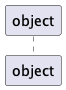
\includegraphics{Immagini/test-2.png}
  \caption{Object}
\end{figure}

\subsection{Attribute}
In particularly in Class Diagrams attributes are the constituting elements of a class. Multiple class could have the same attributes, if two class have the same attributes but different names, most of the time they could be identify by the same class hence being the same thing. Attributes have types that can be user defined (via enumerations) or simply have types define into the UML standard. They optionally can be multiple or single attributes(having multiple phone numbers in a class defining a person). Attributes can optionally have the \emph{\{ID\}} notation, which in class diagrams related to databases identify the primary key of the class(table).
\subsection{Operation}
An Operation is a BehavioralFeature that may be owned by an Interface, DataType or Class. Operations may also be templated and used as template parameters.

\subsection{Associations}
An association describes a semantic dependency between two classes. The semantics dependency can range from simple message passing to enclosing one class within another. The details of the semantic dependency may not be explicit in the diagram.\\

 Each association may optionally have a label. Though unnamed associations are somewhat vague for the designers and implementers, UML does not require a label for an association. If present, the label of an association uniquely determines the association itself.\\ 
 
 An association is generally uni-directional; the direction of the association is implied by the meaning of the label; so, the designer is expected to choose a suitable name for the association that is meaningful in the current application.\\
 
 An arrow is attached to the association label or to one end of the association in order to indicate the direction explicit.\\
 
 An association must connect exactly two classes; it is possible for an association to connect the same class on either end in which case it is called a recursive association.\\
 
  There can be any number of distinct associations between the same pair of classes. An association may optionally have a cardinality on either end of the association. A cardinality symbol (also called multiplicity in UML) is of the form 'n..m' where n and m are numbers, n >= 0, m >= 0 and m >= n.\\
  
  When an association from a class A to B has a cardinality of n..m at the end close to the class B, it is read as "every object of class A is associated with n to m objects of class B at the same time". The symbol '*' can also be used in place of 'n..m', which means 'zero or more'.\\
  
  An association may optionally have a role. A role symbol is a label close to the participating class. Consequently, each class in the association may have a role.\\
  An association may optionally have one or more constraints enclosed in curly brackets and placed near the association. Sometimes, the constraints may be imposed on more than one association. 
\subsection{Multiplicity}
Describes how many instances of one class can be connected to an instance of another class through a given association. This relation is often expressed as a string showing the lower and upper bounds at the endpoints of a connection.

\subsection{Generalization}
TA Generalization is a taxonomic relationship between a more general Classifier and a more specific Classifier. Each instance of the specific Classifier is also an instance of the general Classifier. The specific Classifier inherits the features of the more general Classifier. A Generalization is owned by the specific Classifier.
\subsection{Aggregation}
 An aggregation relationship between a pair of classes indicates that an object of one class encloses an object of the other class. The class at the diamond end of the aggregation symbol is an aggregate and the other class is a component. For example, the class "Polygon" aggregates the class "Line", in which case the diamond end of the aggregation symbol must touch the class "Polygon". An aggregation is also an association; however, there are some differences.
\subsection{Composition}
Is exactly like Aggregation except that the lifetime of the 'part' is controlled by the 'whole'. This control may be direct or transitive. That is, the 'whole' may take direct responsibility for creating or destroying the 'part', or it may accept an already created part, and later pass it on to some other whole that assumes responsibility for it.